\documentclass[aspectratio=169]{beamer}

\usetheme[titleformat=allcaps,sectionpage=simple,progressbar=frametitle,background=dark]{metropolis}
\RequirePackage{etoolbox}
\RequirePackage{ifxetex}
\RequirePackage{ifluatex}
\RequirePackage{pgfopts}

\usepackage{color}
\definecolor{background}{HTML}{ffffff}
\definecolor{text}{HTML}{333333}
\definecolor{background}{HTML}{333333}
\definecolor{text}{HTML}{ffffff}
\definecolor{warning}{HTML}{f0ad4e}
\definecolor{success}{HTML}{5cb85c}

\setbeamercolor{progress bar}{fg=success,bg=background}
\setbeamercolor{progress bar in section page}{fg=success,bg=background}
\setbeamercolor{title separator}{fg=warning,bg=text}
\setbeamercolor{normal text}{fg=text,bg=background}
\setbeamercolor{frametitle}{fg=text,bg=warning}
\setbeamercolor{section title}{fg=text,bg=warning}
\setbeamercolor{palette primary}{bg=warning}

\setbeamercolor{titlelike}{fg=text}
\setbeamercolor{author}{fg=text}
\setbeamercolor{date}{fg=text}
\setbeamercolor{institute}{fg=text}

%\usepackage{default}
\usepackage{graphicx}
\usepackage{amssymb}
\usepackage[ngerman,english]{babel}
\usepackage{appendixnumberbeamer}

\usepackage{pgfpages}
%\setbeameroption{show notes on second screen}

% Define block styles
\tikzstyle{decision} = [diamond, color=background, fill=red!20, text width=5em, text badly centered]
\tikzstyle{block} = [rectangle, color=background, fill=blue!20, text width=7em, text centered, rounded corners, minimum height=4em, text centered]
\tikzstyle{cloud} = [ellipse, color=background, fill=green!20, minimum height=2em, text centered, text width=4em]

\title{Interpolation - On the example of the intra-urban Heat island effect in Berlin}
\subtitle{FOSSGIS Seminar}
\date{Janurary 27, 2021}
\author{Anja Doppelmayr \& Malte Heinzelmann}
\institute{Ruprecht-Karls-Universit\"at Heidelberg}

\makeatletter
\def\beamer@framenotesbegin{% at beginning of slide
	\usebeamercolor[fg]{normal text}
	\gdef\beamer@noteitems{}%
	\gdef\beamer@notes{}%
}

\setlength{\metropolis@titleseparator@linewidth}{2pt}
\setlength{\metropolis@progressonsectionpage@linewidth}{2pt}
\setlength{\metropolis@progressinheadfoot@linewidth}{2pt}

\newlength\beamerleftmargin
\setlength\beamerleftmargin{\Gm@lmargin}
\makeatother

\usepackage[export]{adjustbox} 

\usepackage{tikz}
\usetikzlibrary{arrows,positioning,shapes,arrows.meta}

\usepackage[absolute,overlay]{textpos}
\setlength{\TPHorizModule}{\paperwidth} % horizontal unit
\setlength{\TPVertModule}{\paperheight} % vertical unit

\usepackage[
backend=biber,
style=alphabetic,
]{biblatex}

\addbibresource{../writeup/biblatex.bib} %Imports bibliography file

\newenvironment*{env}{}{}

\begin{document}
	\begin{frame}[plain]
		\makebox[0pt][l]{%
			\hspace*{-11mm}
			%\hspace*{-\beamerleftmargin}
			\raisebox{-\totalheight}[0pt][0pt]{%
				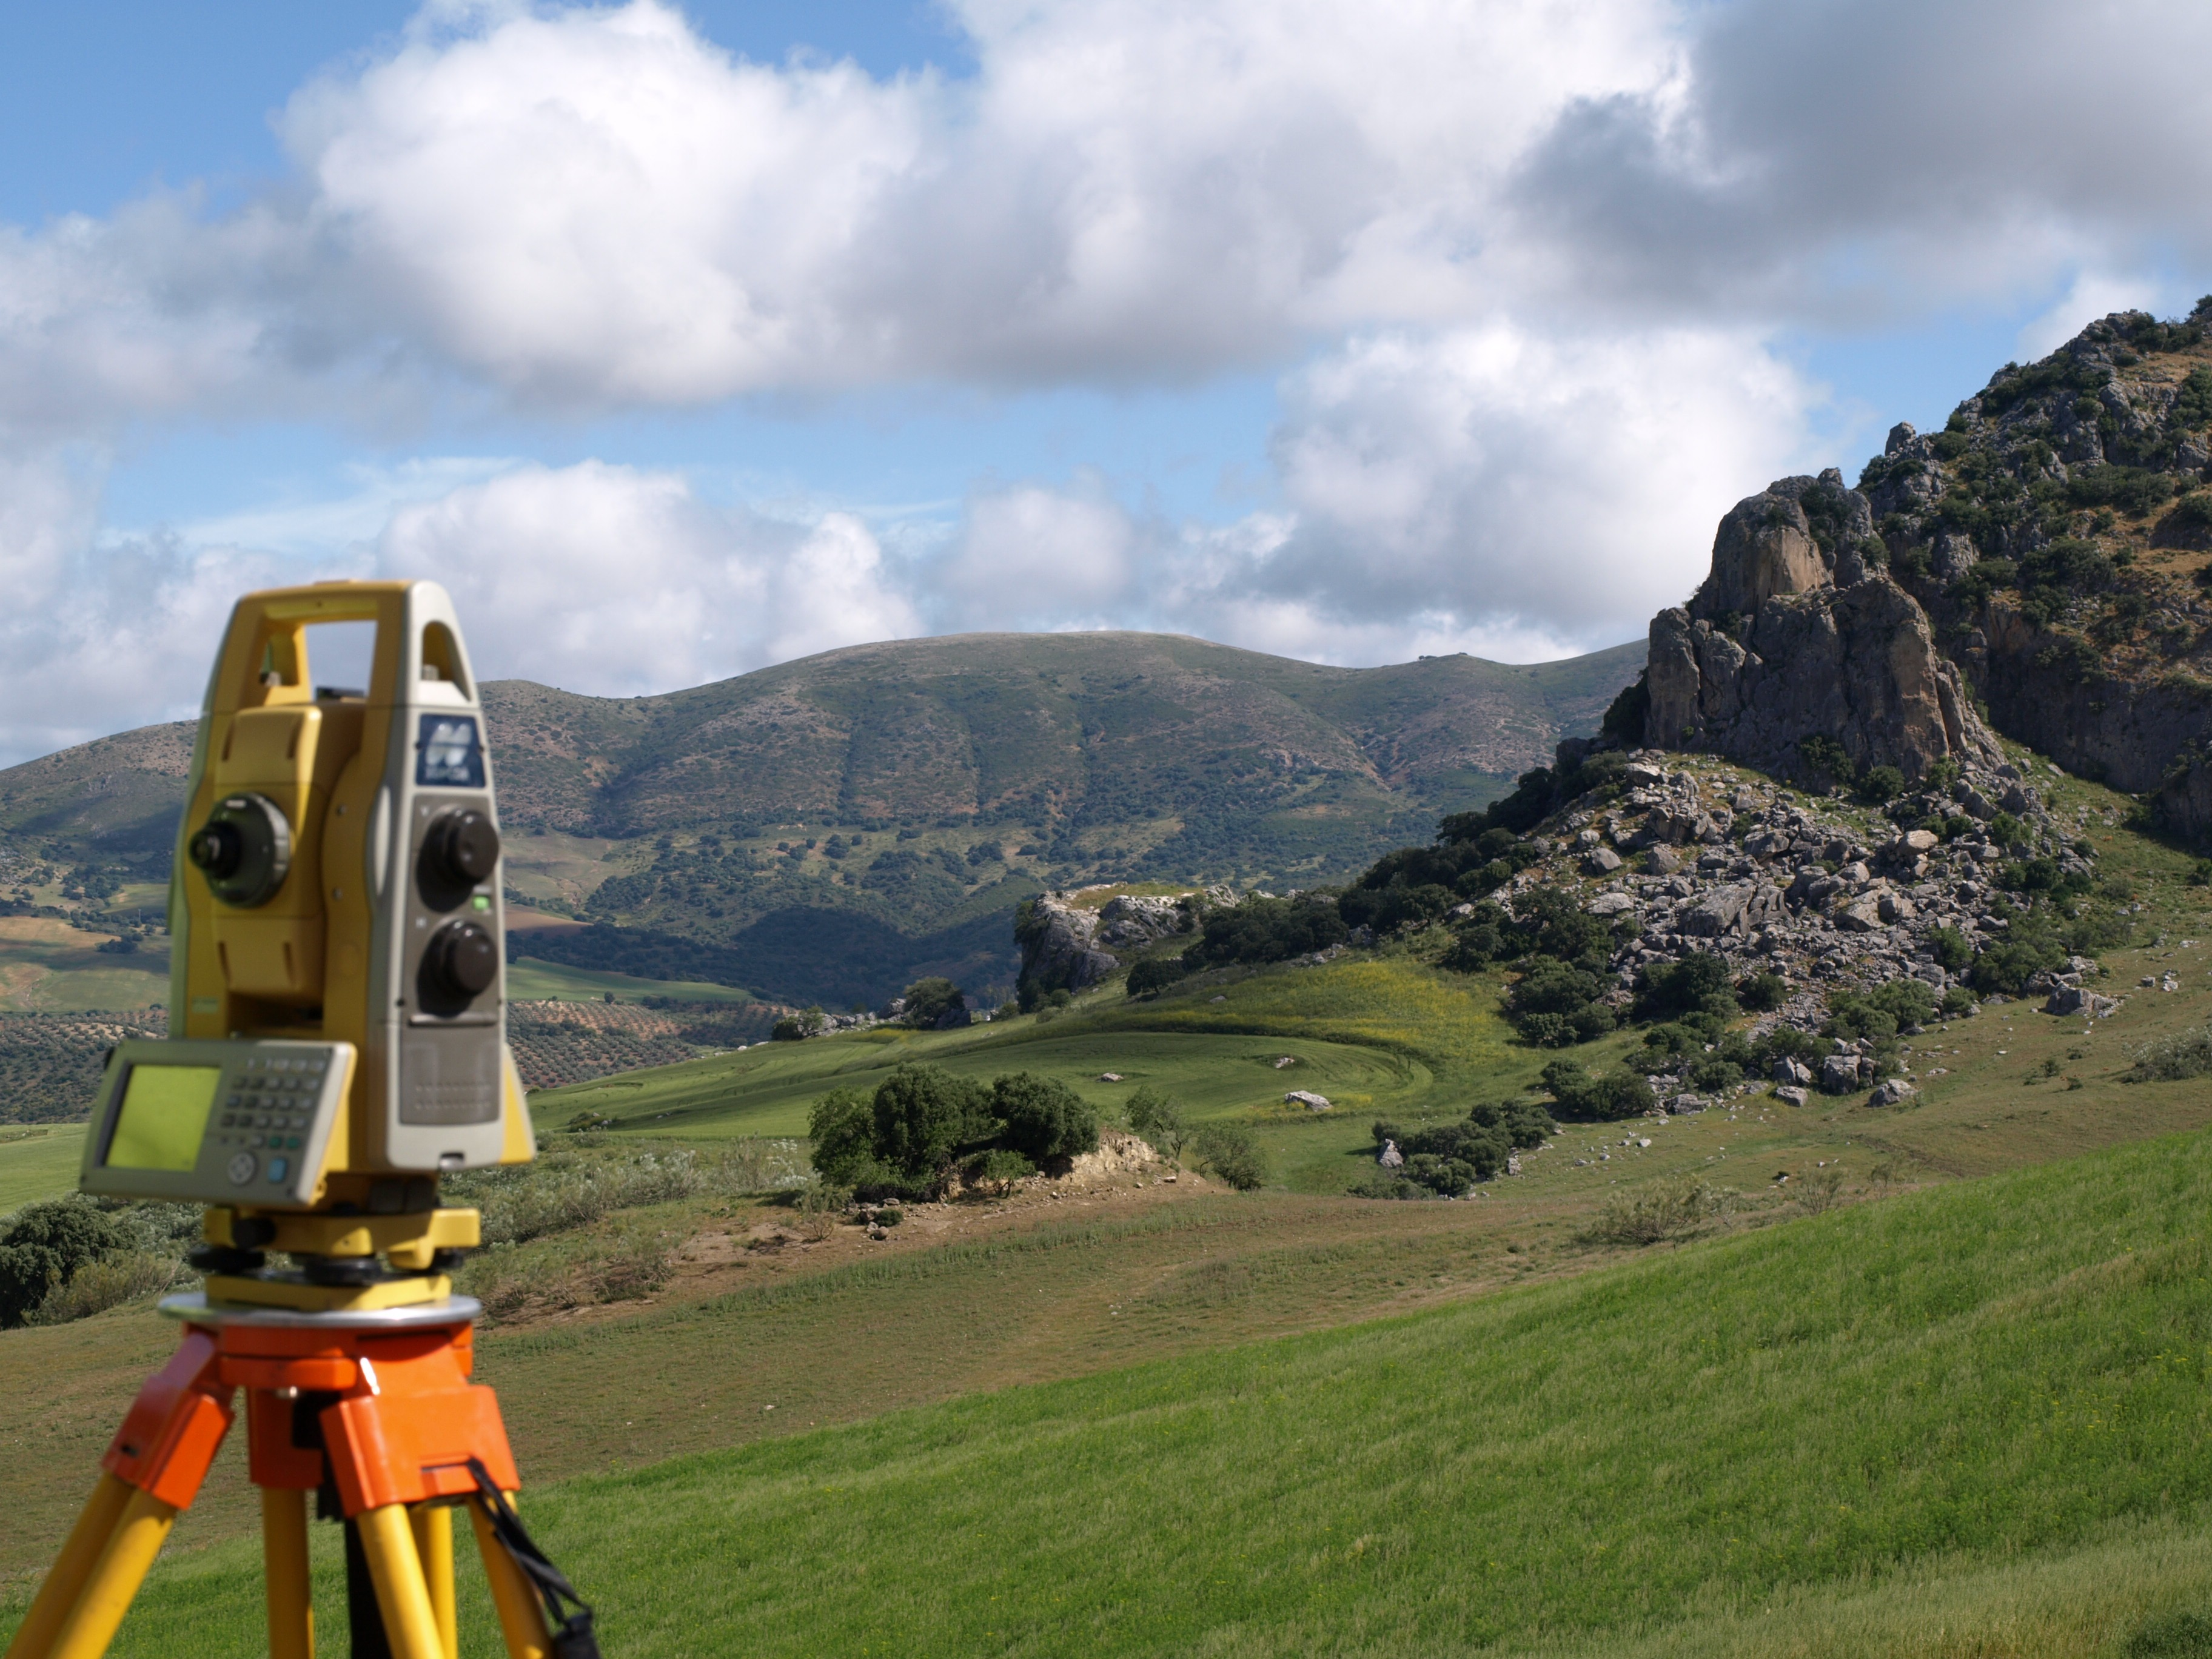
\includegraphics[width=\paperwidth,keepaspectratio]{images/background}
			}
			\hspace*{-\paperwidth}
			\hspace*{-5mm}
			\raisebox{-\totalheight}[0pt][0pt]{%
				
\includegraphics[width=\paperwidth,height=\paperheight]{images/backdrop.png}
			}
		}
		\begin{textblock}{1}[1,1](0.995,0.99)
			\setlength\topsep{0pt}
			\begin{flushright}
				\tiny\color{text} Source: Pixabay (davidph, topography-station-measurement-202278)%
			\end{flushright}
		\end{textblock}
		\titlepage
	\end{frame}

	\begin{frame}{Agenda}
		\tableofcontents[]
	\end{frame}

	% !TeX root = ../presentation.tex

\section{Introduction}
\begin{frame}{What is interpolation?}
	\begin{columns}[T] % align columns
		\begin{column}{.48\textwidth}
			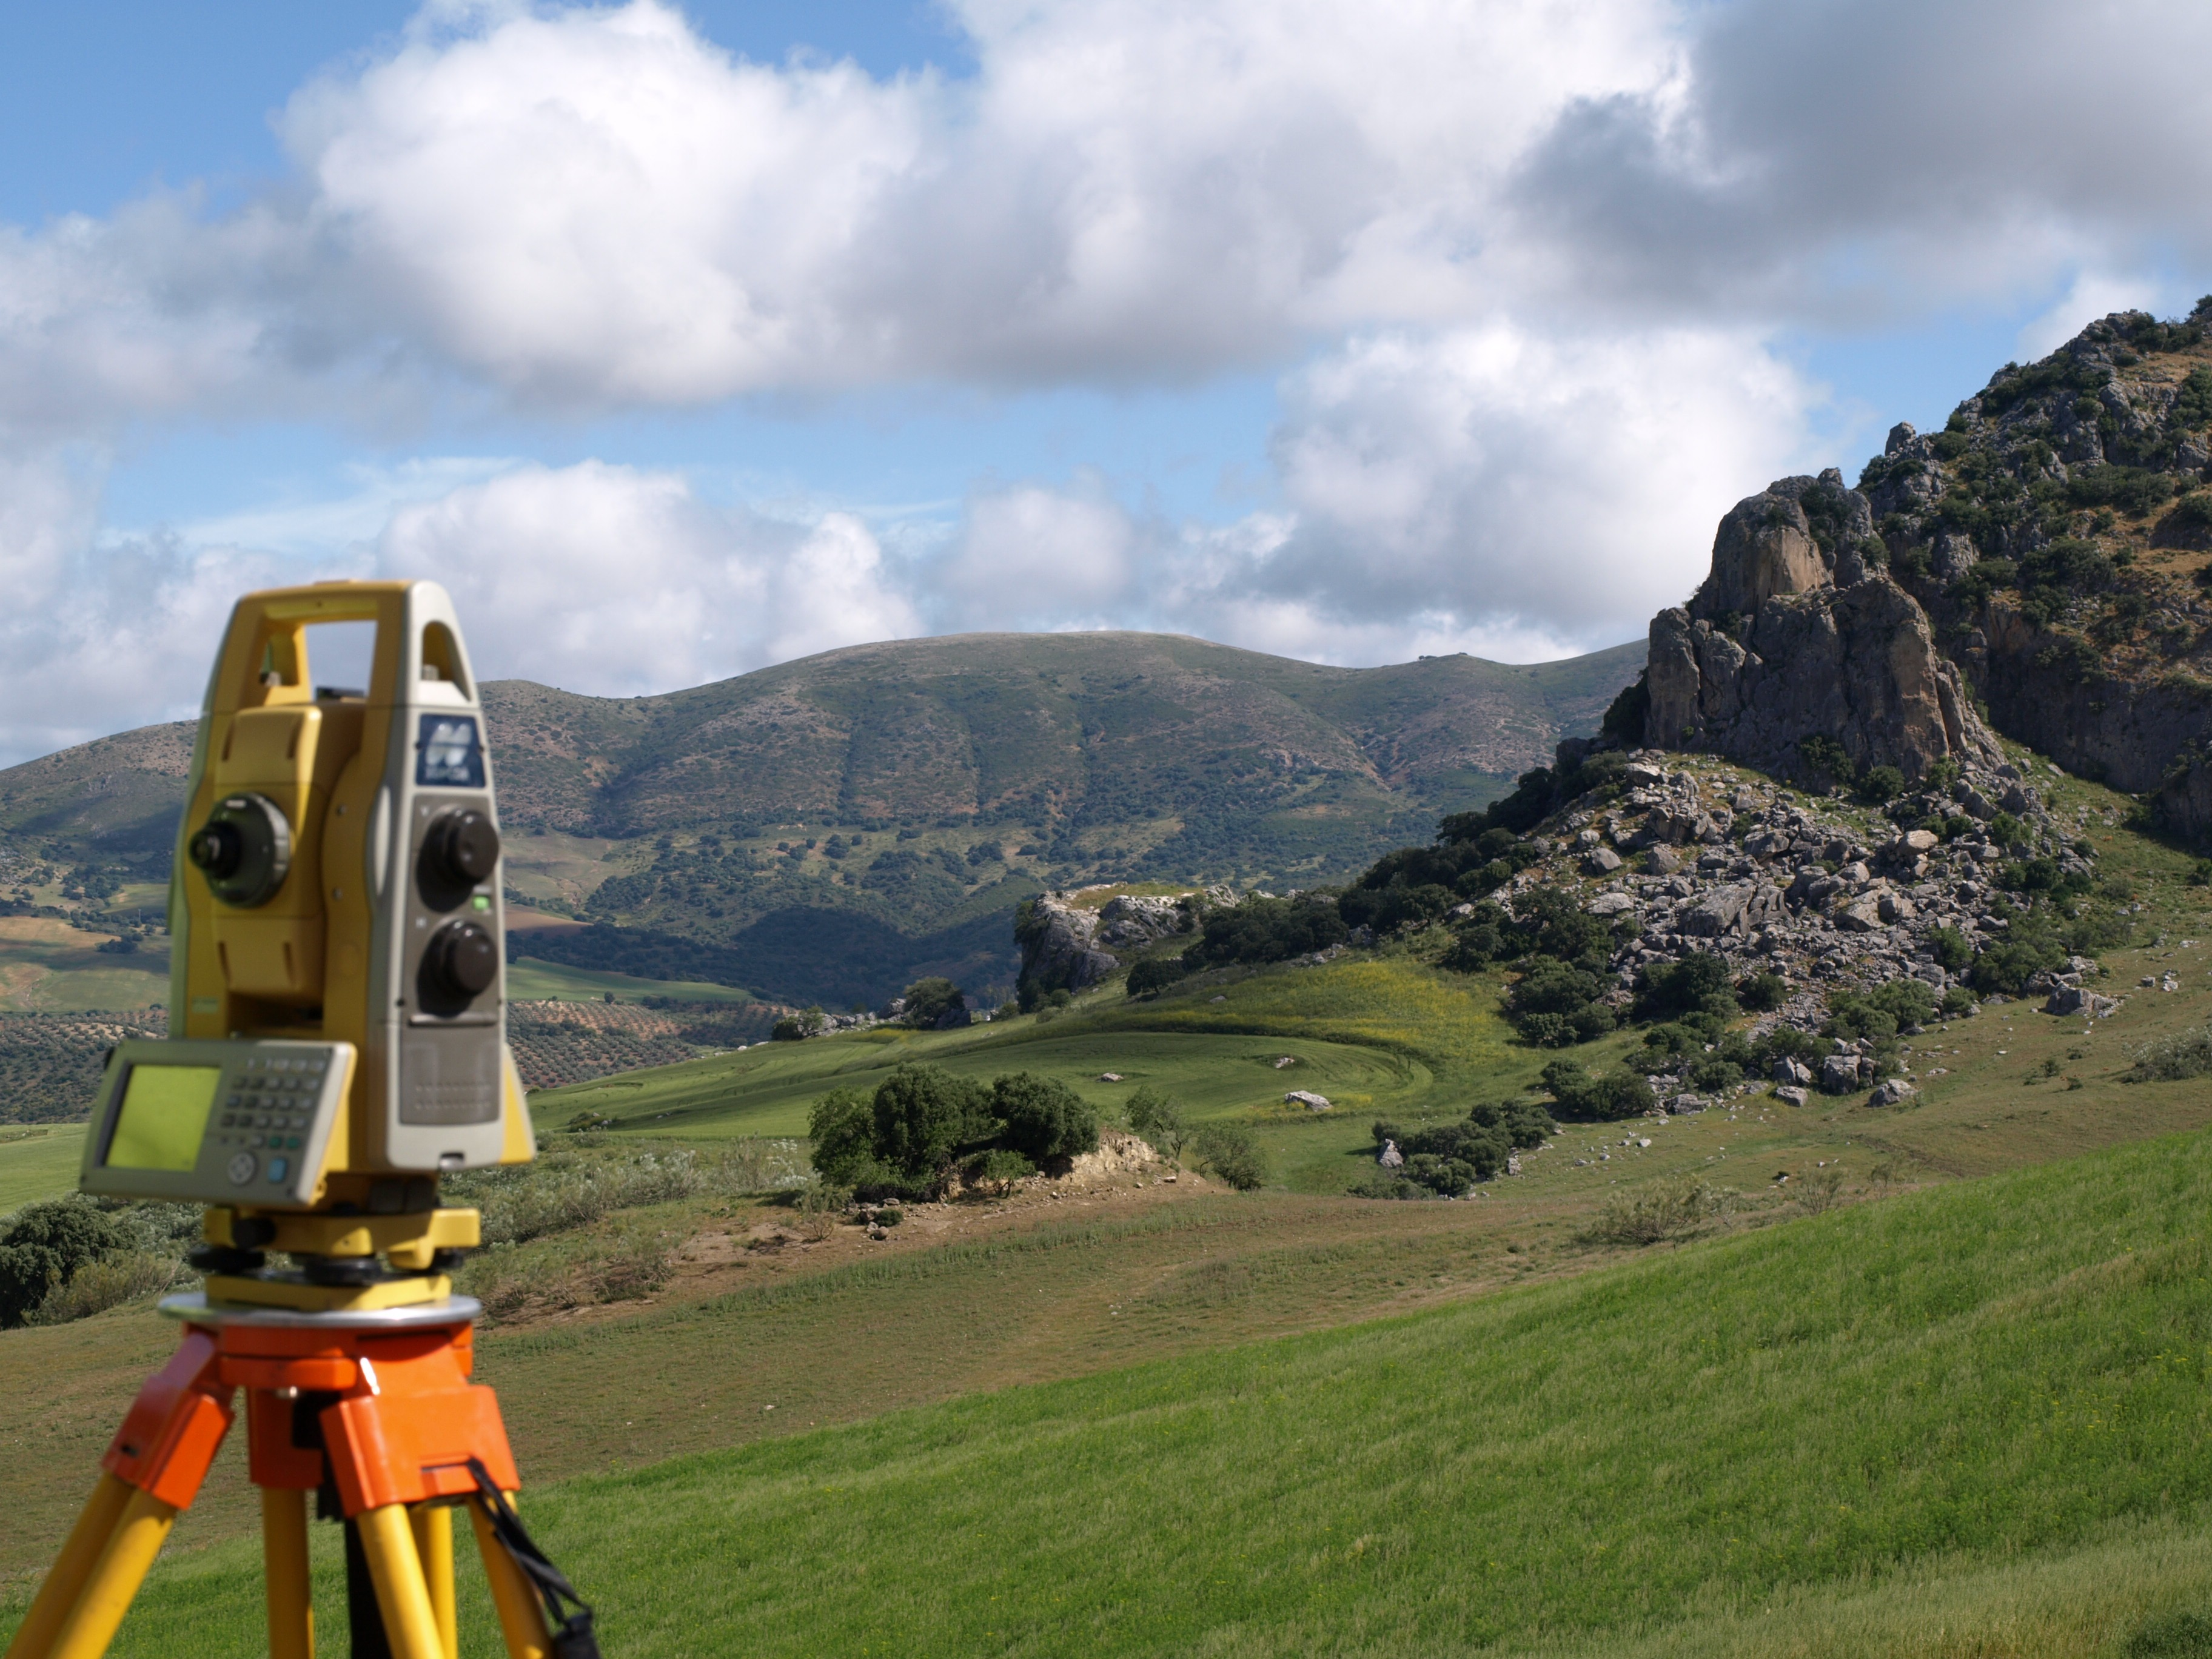
\includegraphics[width=\linewidth]{images/background}
		\end{column}%
		\hfill%
		\begin{column}{.56\textwidth}
			\begin{itemize}
				\item TODO
				\item TODO 2
			\end{itemize}
		\end{column}%
	\end{columns}
	\note{say "hello" now}
\end{frame}
\begin{frame}{This is interpolation!}
\begin{columns}[T] % align columns
	\begin{column}{.56\textwidth}
		\begin{itemize}
			\item TODO
		\end{itemize}
	\end{column}%
	\hfill%
	\begin{column}{.48\textwidth}
		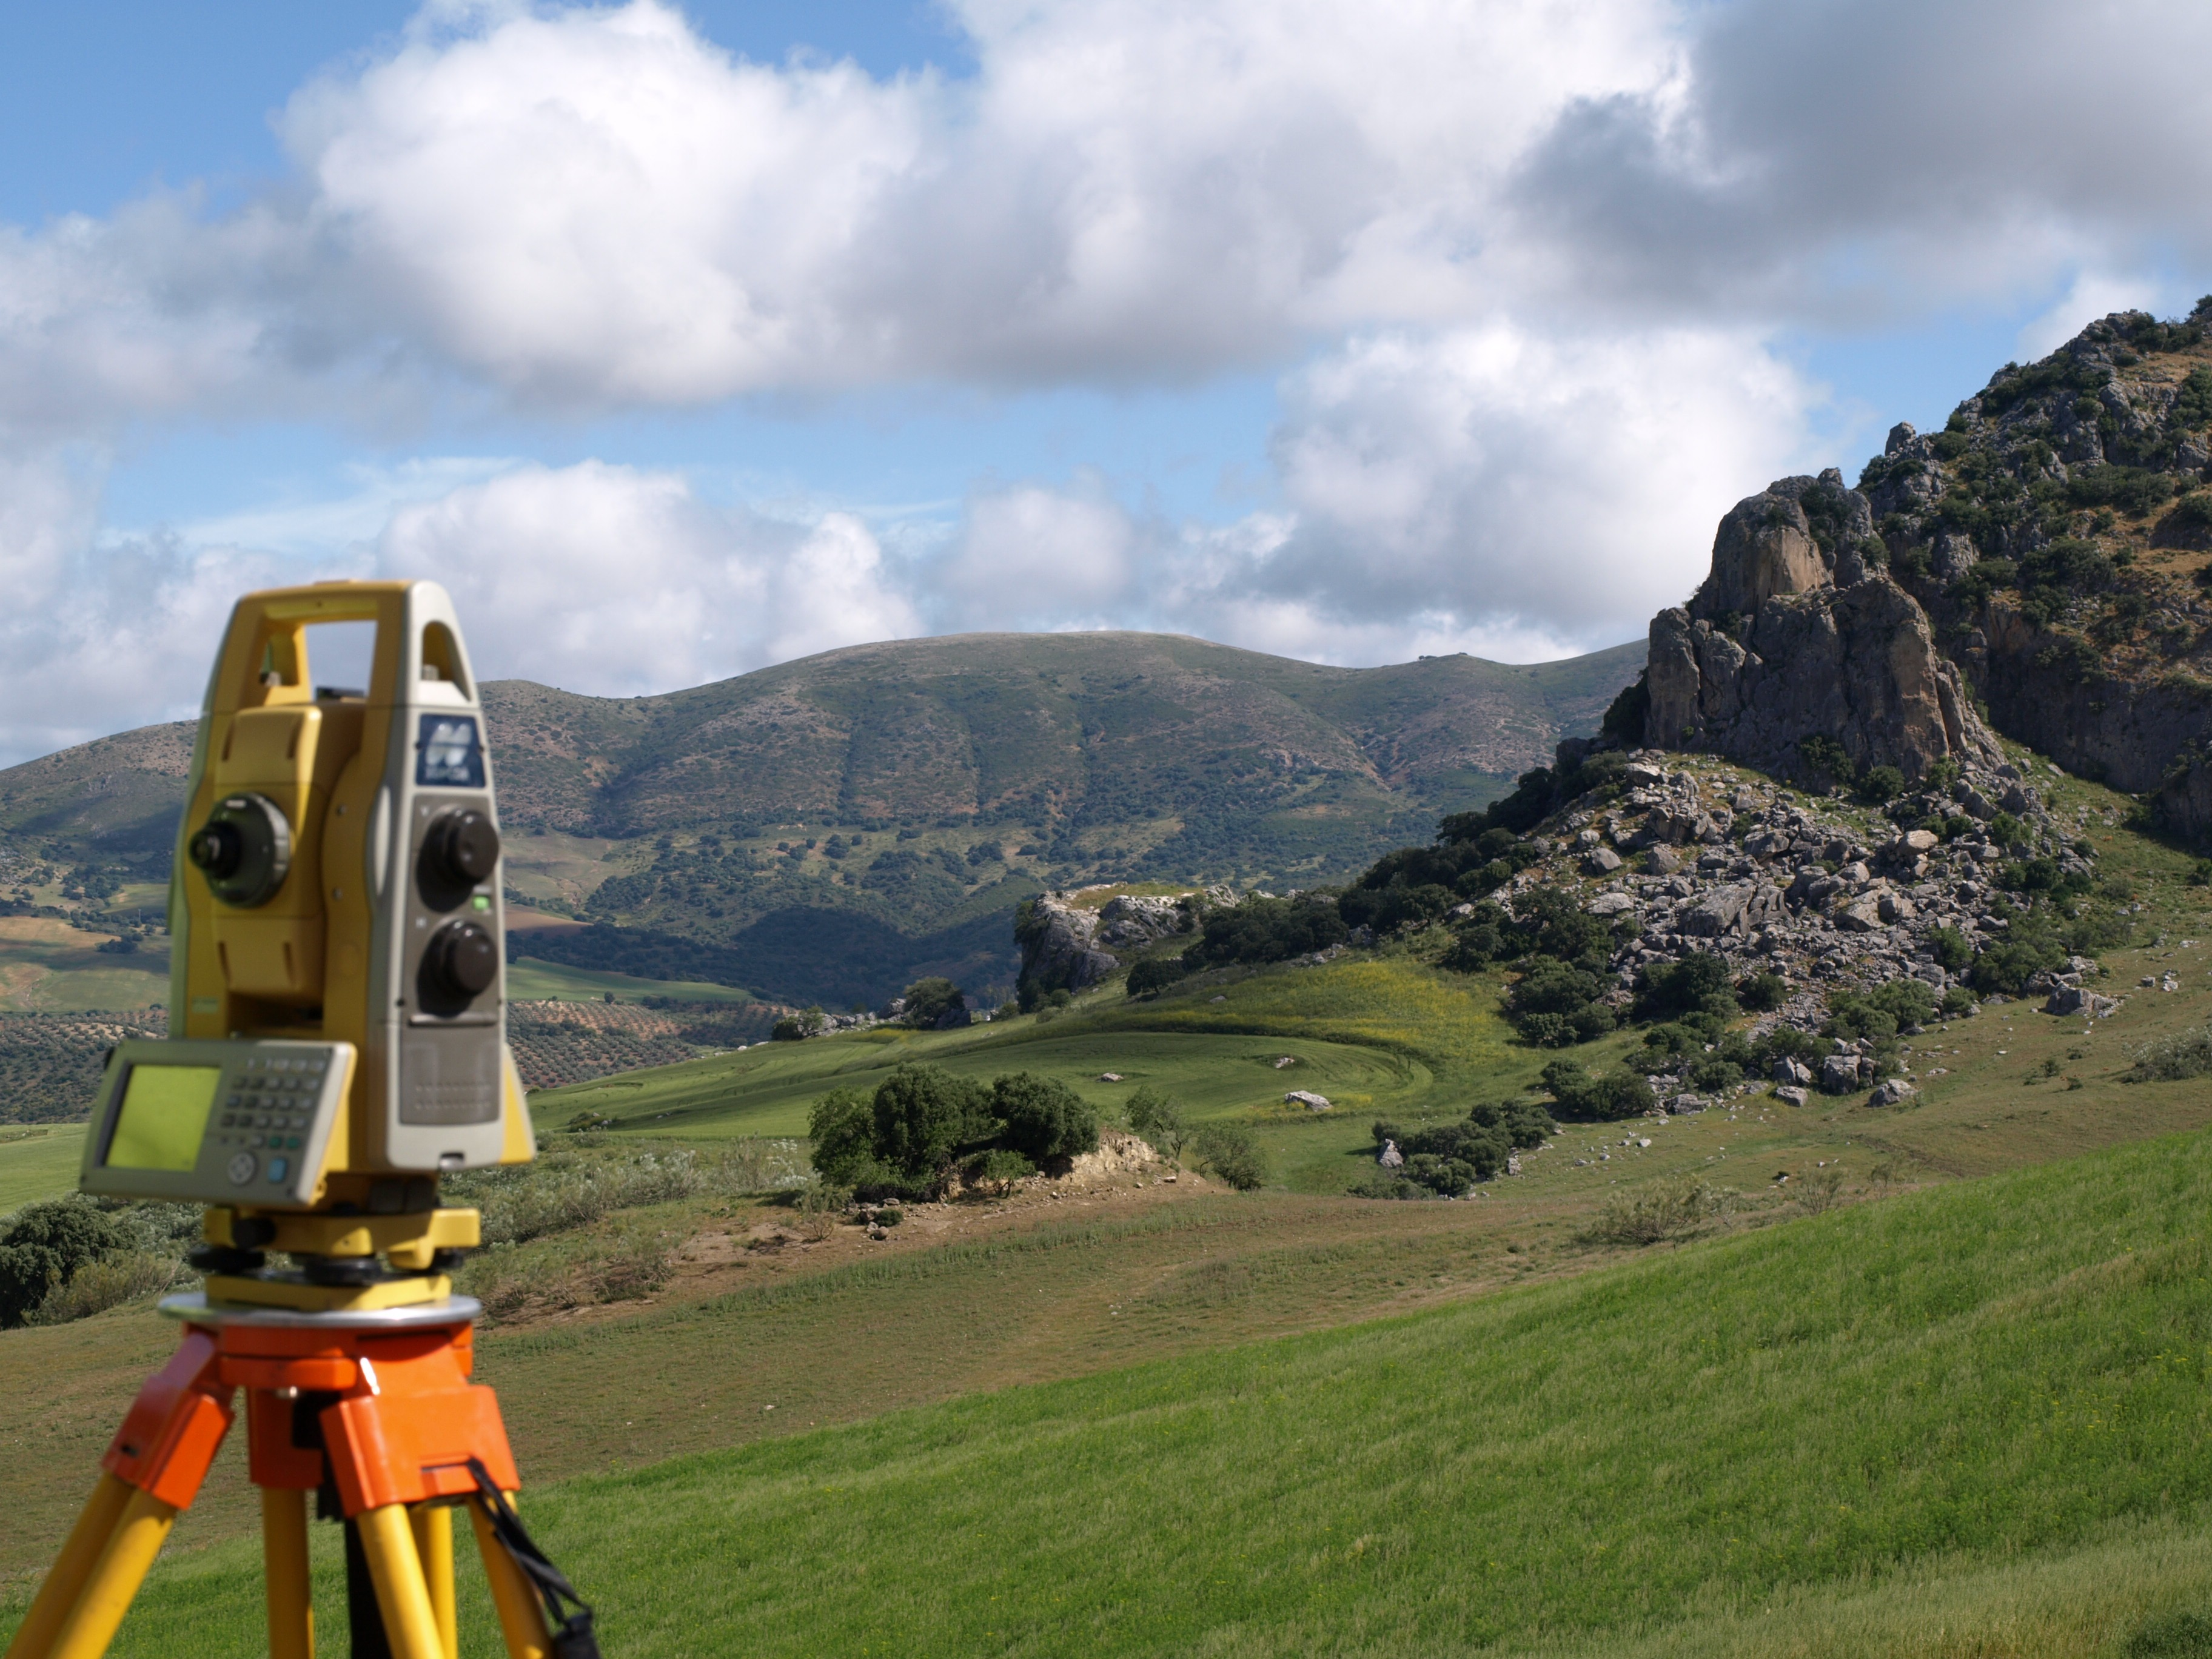
\includegraphics[width=\linewidth]{images/background}
	\end{column}%
\end{columns}
\note{say "hello" now}
\end{frame}

	% !TeX root = ../presentation.tex

\section{Heat Island Effect}
\begin{frame}{What is the heat island effect?}
	\begin{columns}[T] % align columns
		\begin{column}{.48\textwidth}
			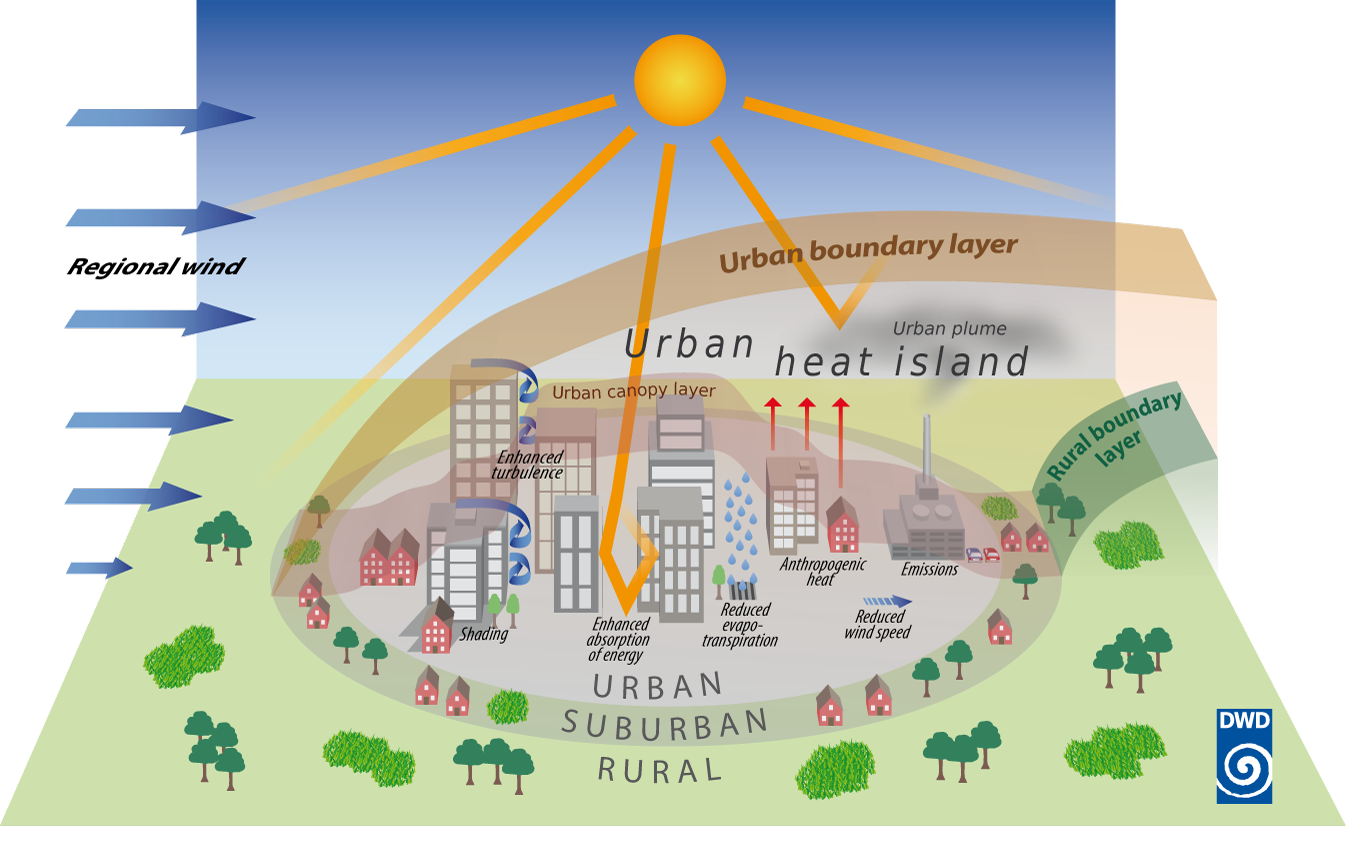
\includegraphics[width=\linewidth]{images/urbanheatisland_01.png}\\
			\textit{\footnotesize Source: Deutscher Wetterdienst\\Urban climate - urban heat islands}
		\end{column}%
		\hfill%
		\begin{column}{.56\textwidth}
			\begin{itemize}
				\item \glqq{}{[\textellipsis]} an urban area or metropolitan area is significantly warmer than its surrounding rural areas due to human activities\grqq{}\footcite{takebayashi_chapter_2020}
				\item Infrastructure, such as buildings, roads and other sealed surfaces absorb and re-emit the sun's radiation in the form of heat
				\item natural landscapes, such as forests and water bodies have a cooling effect\footcite{us_epa_learn_2014}
			\end{itemize}
		\end{column}%
	\end{columns}
	\note{say "hello" now}
\end{frame}
\begin{frame}{This is interpolation!}
	\begin{columns}[T] % align columns
		\begin{column}{.56\textwidth}
			\begin{itemize}
				\item TODO
			\end{itemize}
		\end{column}%
		\hfill%
		\begin{column}{.48\textwidth}
			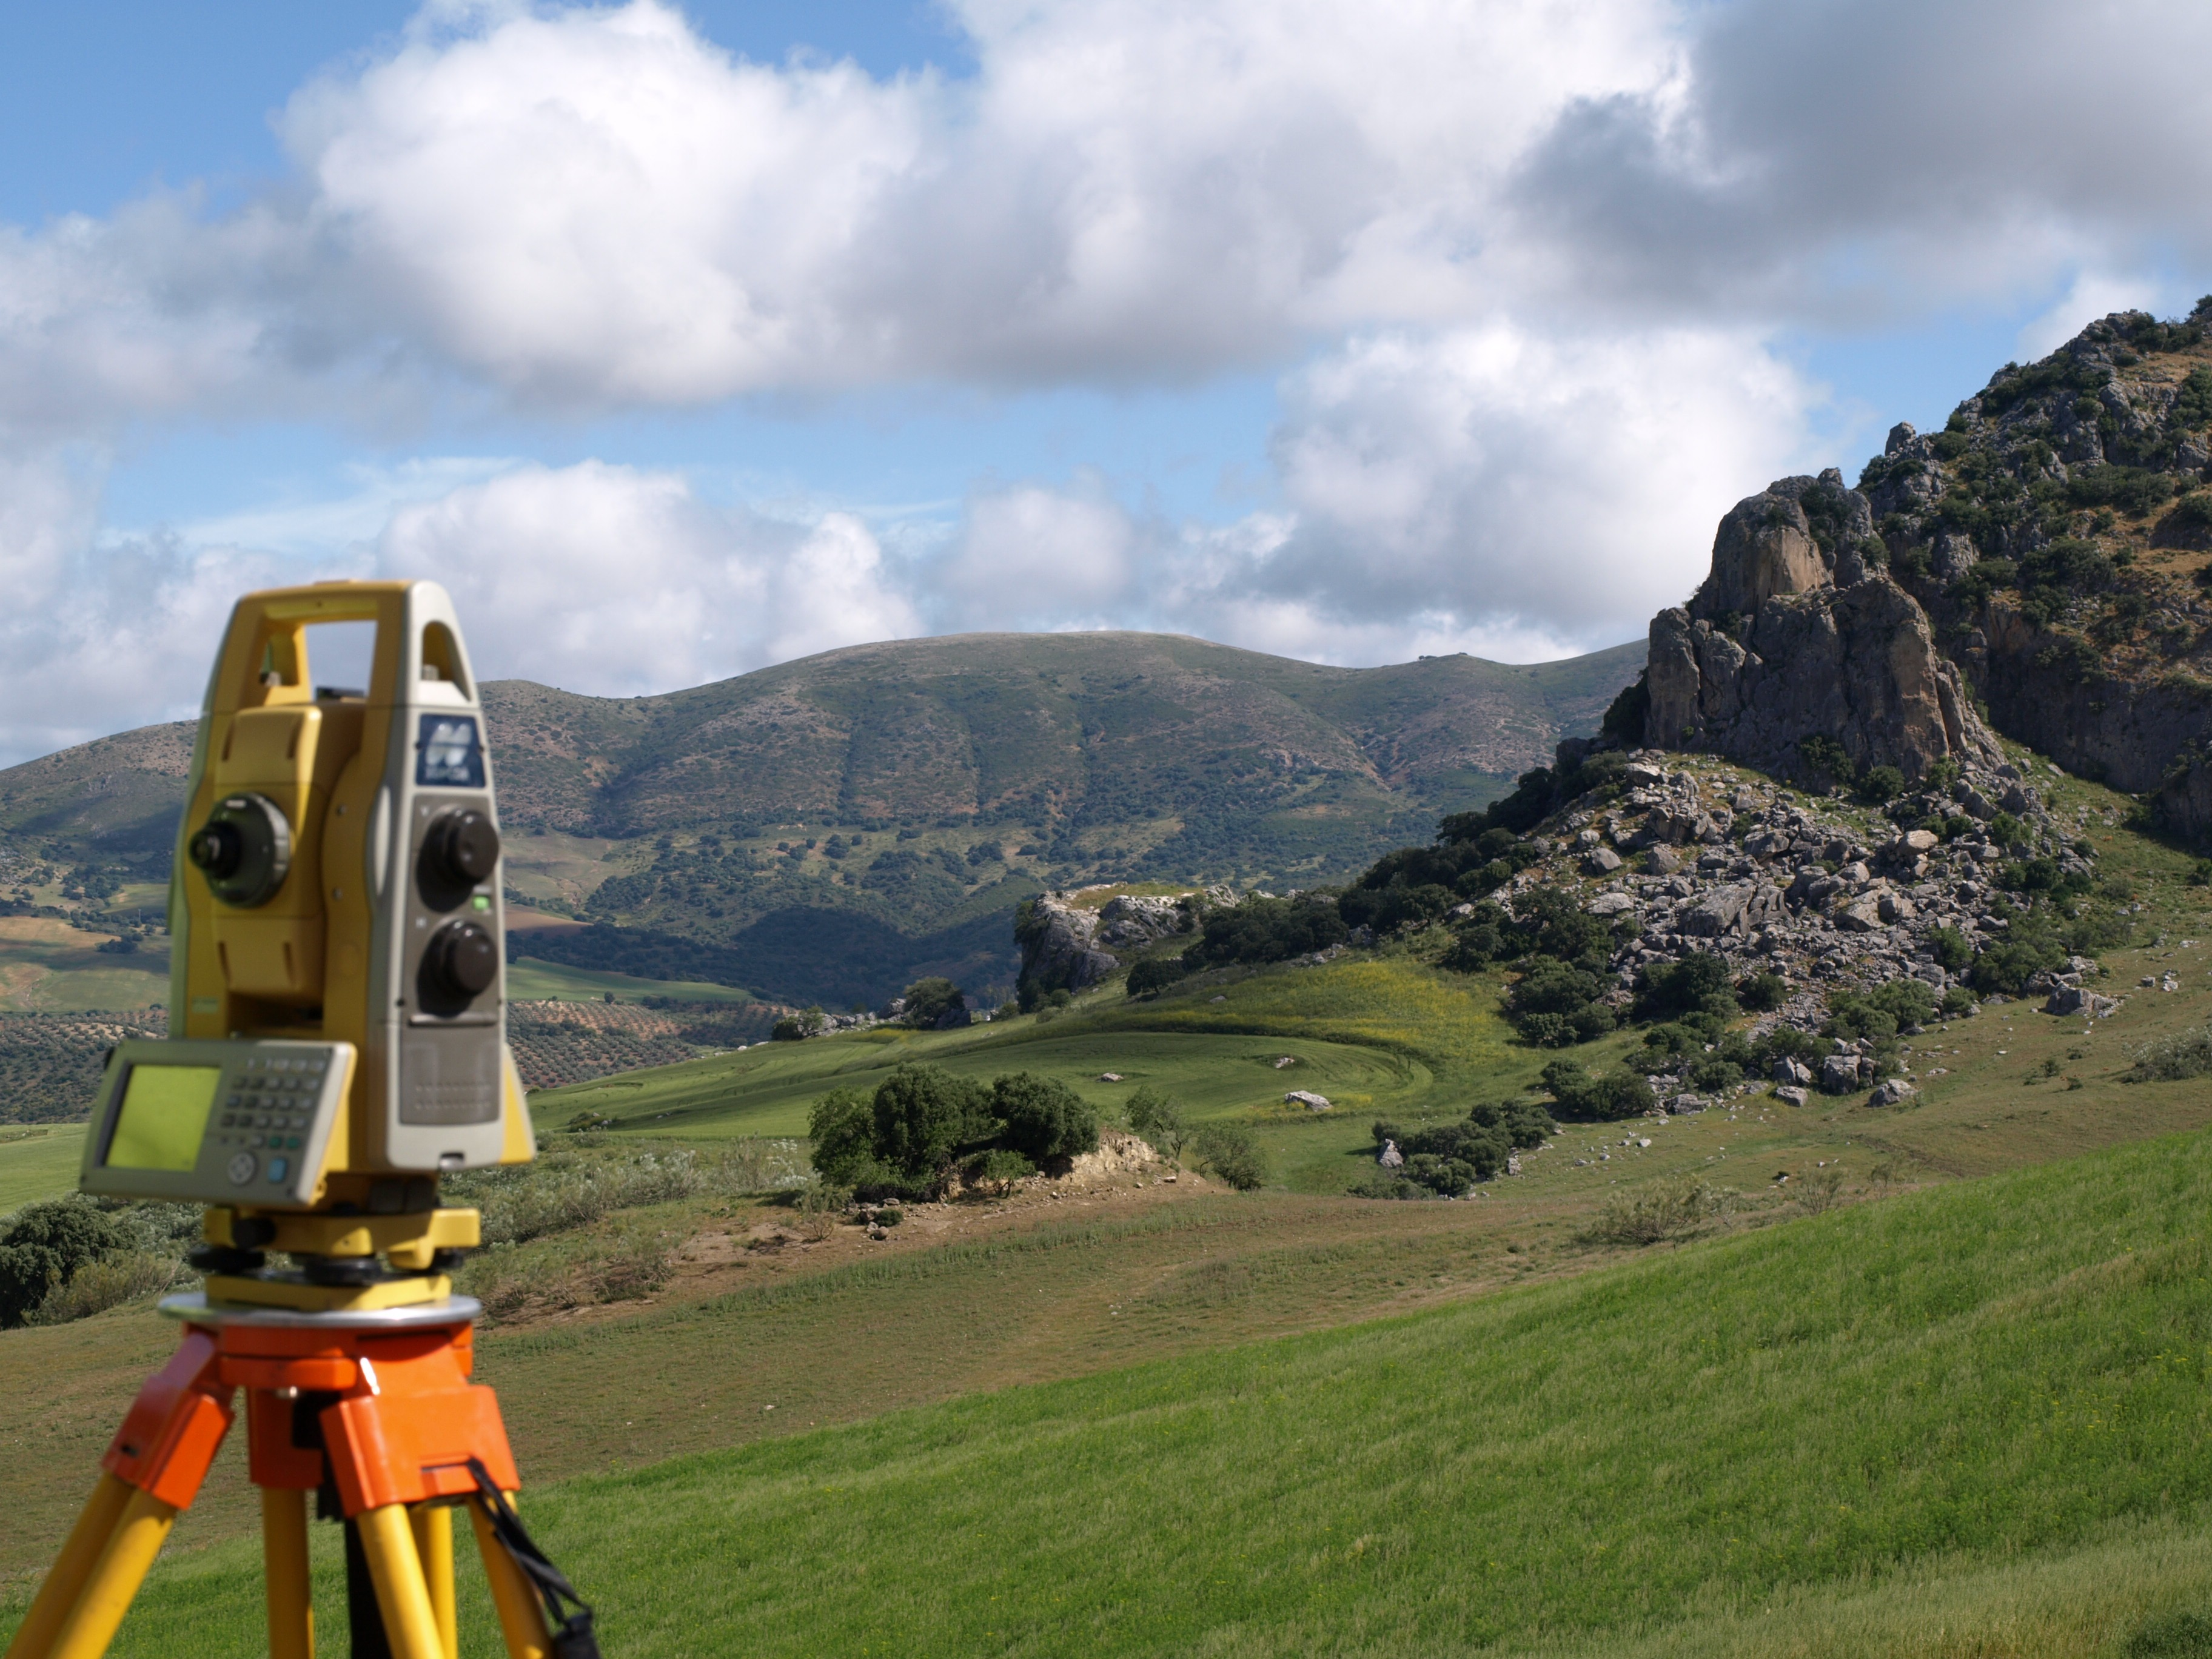
\includegraphics[width=\linewidth]{images/background}
		\end{column}%
	\end{columns}
	\note{say "hello" now}
\end{frame}
	
	% !TeX root = ../presentation.tex

\section{Comparison}
\begin{frame}{Comparison}
	\begin{columns}[T] % align columns
		\begin{column}{.48\textwidth}
			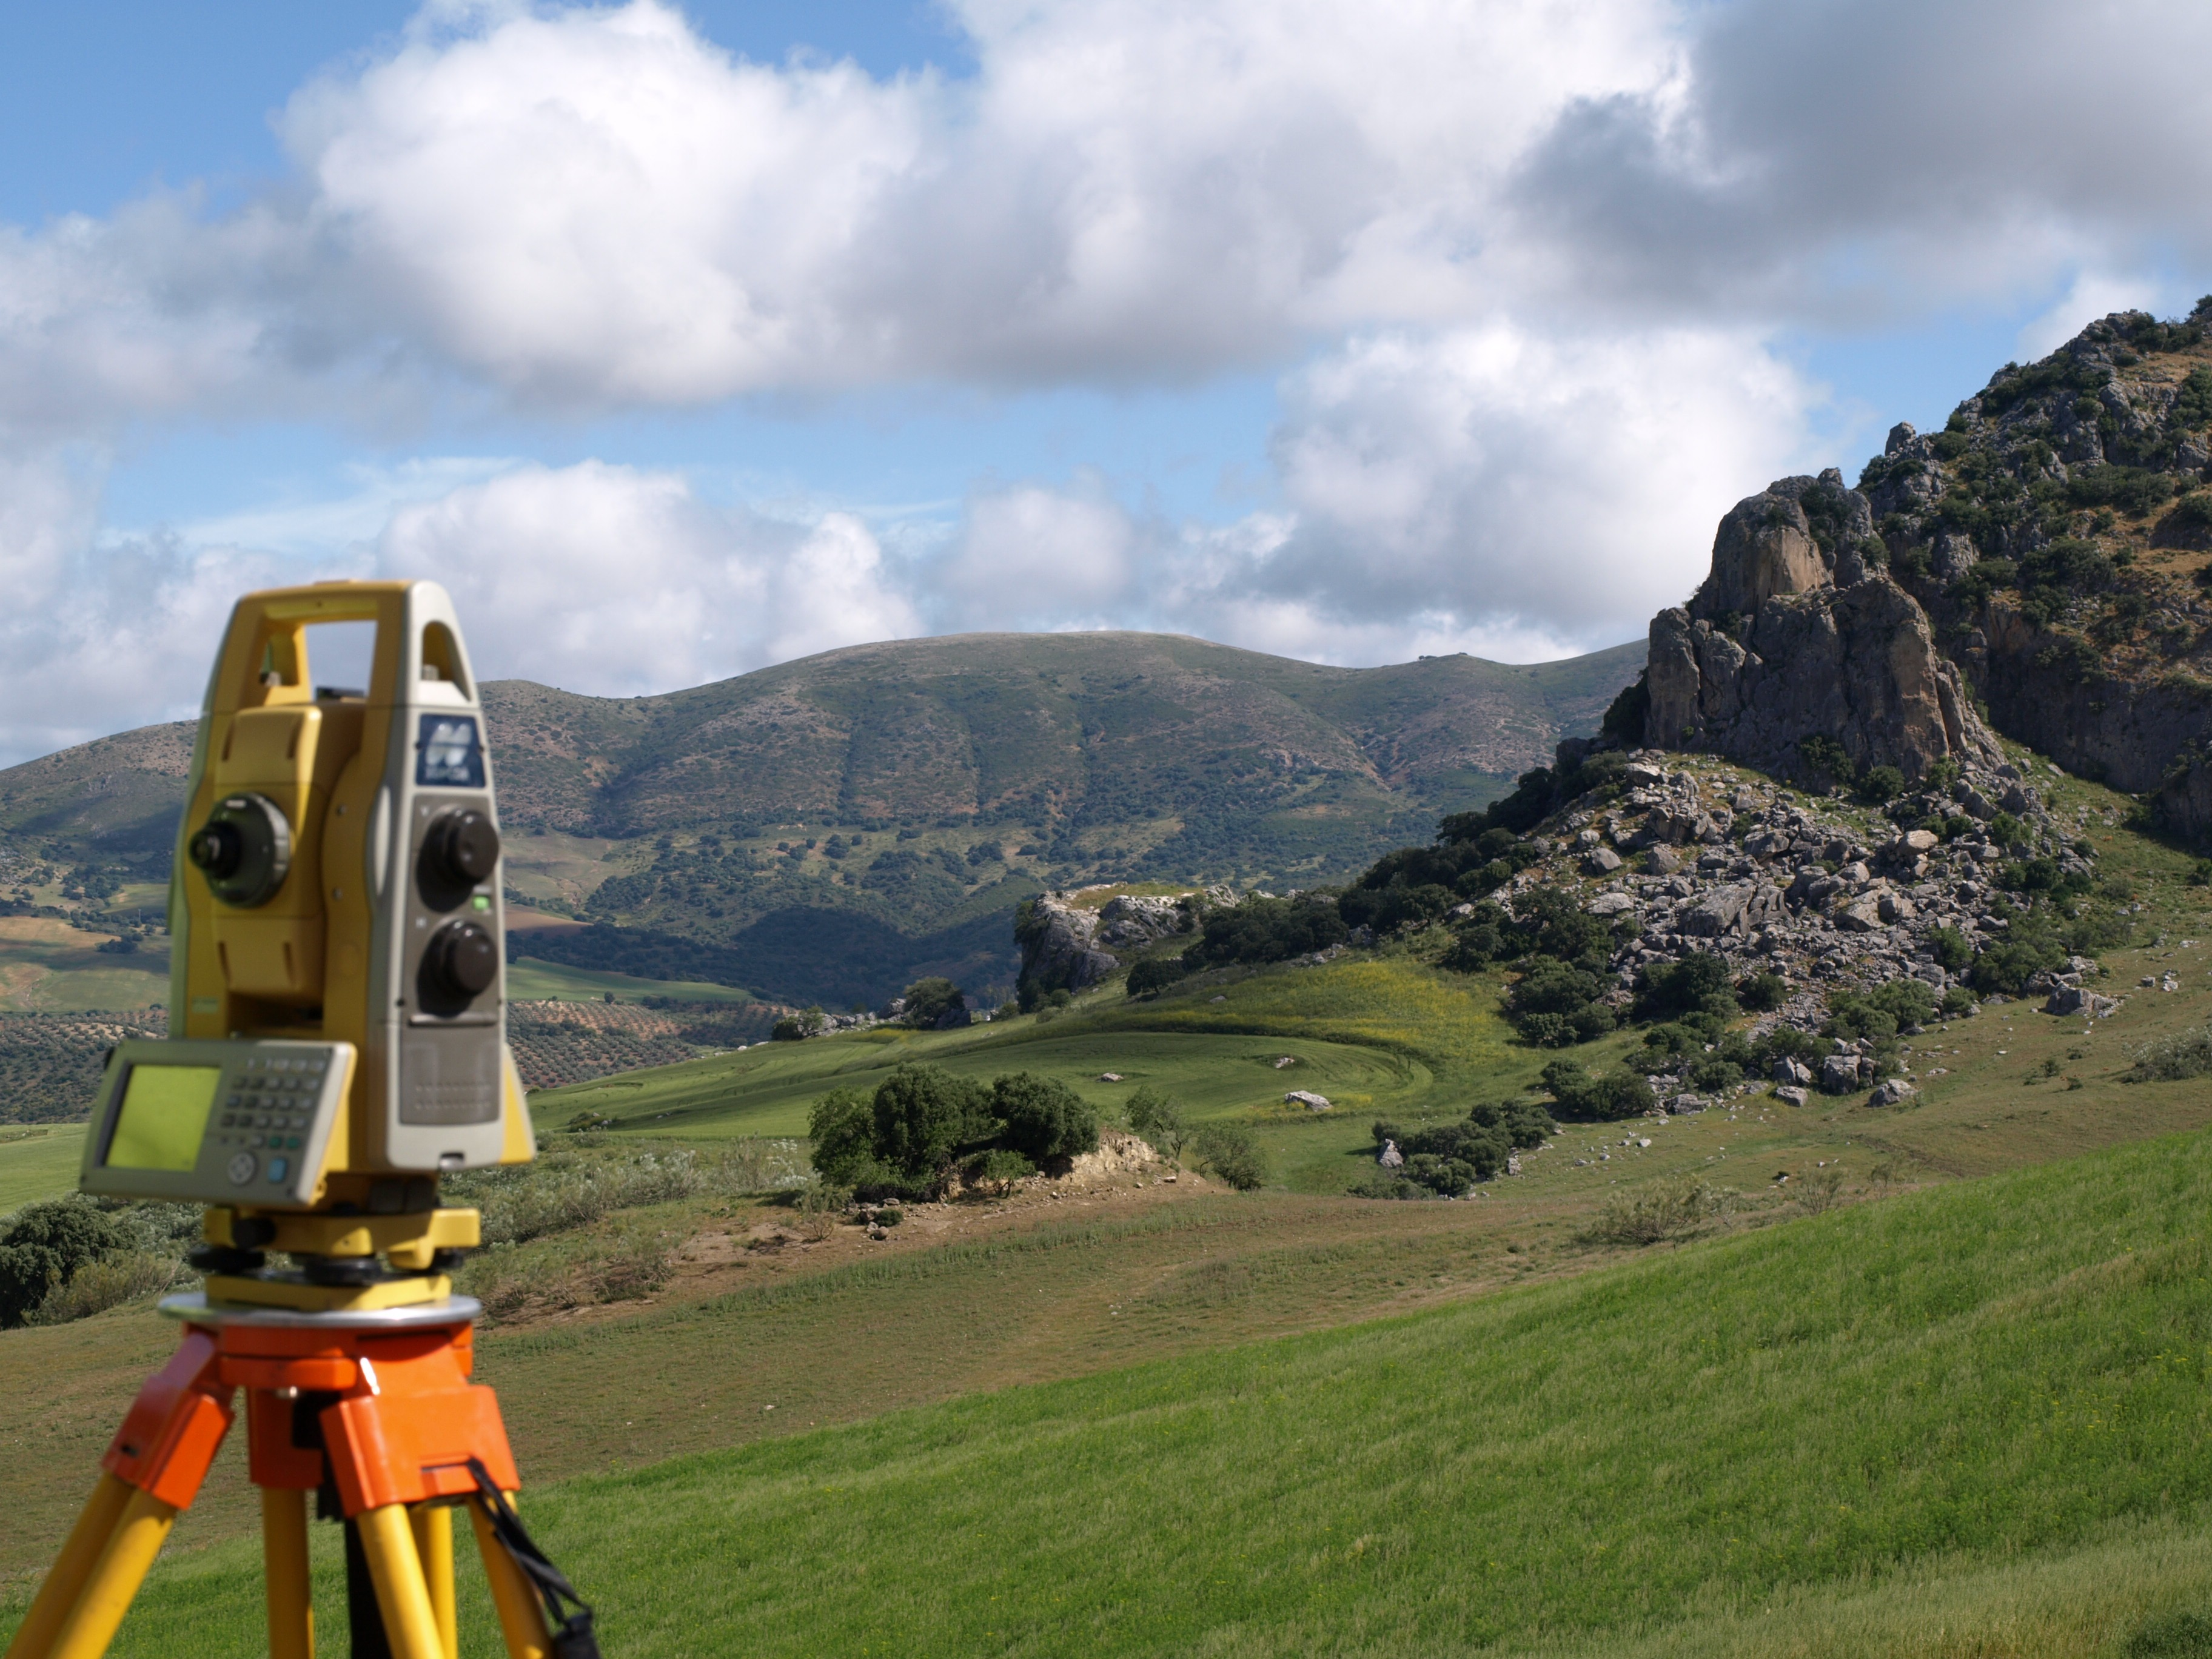
\includegraphics[width=\linewidth]{images/background}
		\end{column}%
		\hfill%
		\begin{column}{.56\textwidth}
			\begin{itemize}
				\item TODO
			\end{itemize}
		\end{column}%
	\end{columns}
	\note{say "hello" now}
\end{frame}
	
	% !TeX root = ../presentation.tex

\section{Results}
\begin{frame}{Results}
	\begin{columns}[T] % align columns
		\begin{column}{.48\textwidth}
			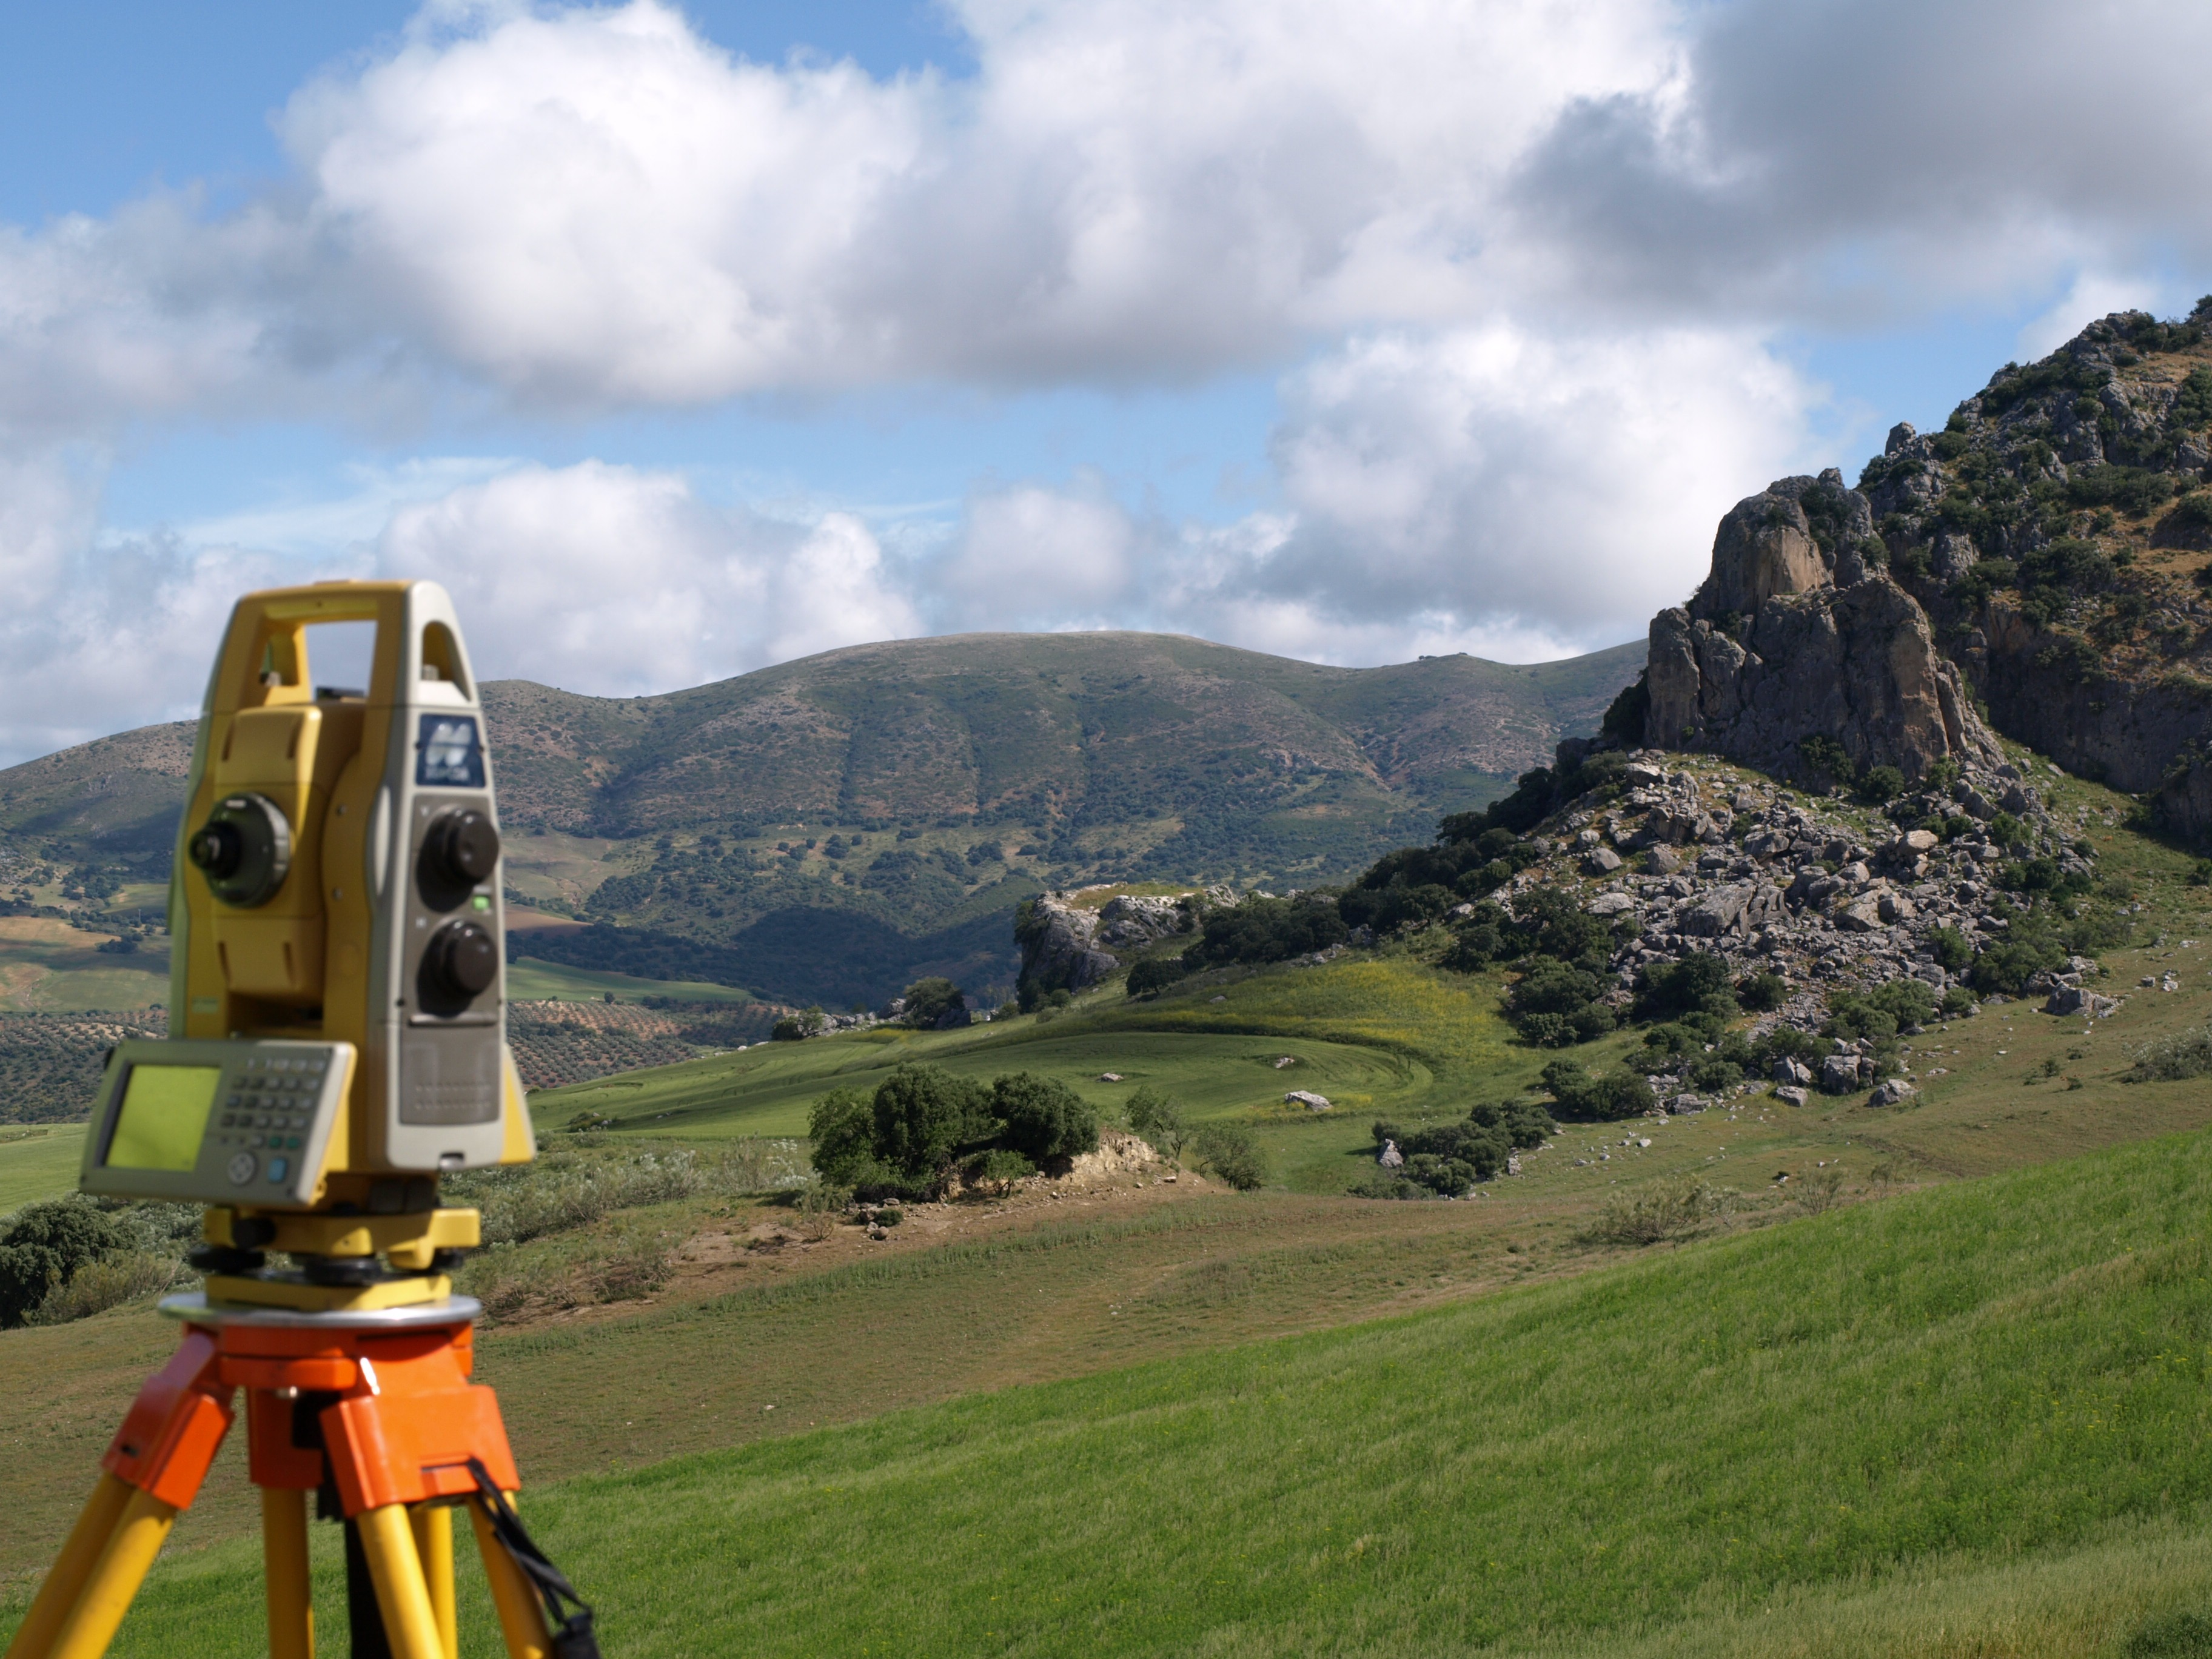
\includegraphics[width=\linewidth]{images/background}
		\end{column}%
		\hfill%
		\begin{column}{.56\textwidth}
			\begin{itemize}
				\item TODO
			\end{itemize}
		\end{column}%
	\end{columns}
	
\end{frame}
	
	% !TeX root = ../presentation.tex

\section{Testing}
\begin{frame}{Testing}
	TODO
\end{frame}
	
	% !TeX root = ../presentation.tex

\section{Discussion}
\begin{frame}{Discussion}
	TODO
\end{frame}
	
	{
		\metroset{sectionpage=none,numbering=none}
		\section{Demo}
		\begin{frame}[standout]
			\begin{env}
				\usebeamercolor[fg]{normal text}
				\LARGE
				DEMO
			\end{env}
		\end{frame}
	}

	% !TeX root = ../presentation.tex

\appendix

\begin{frame}{Appendix}
	TODO
\end{frame}
	
\end{document}
